% % Chapter 2: XAFS Simulations
% % Chapter 2: XANES
% \textit{In this section, I can write about XANES to a super in-depth extent, and likely the bulk of this chapter will be about FEFF and FDMNES theoretical calculations}
% \section{Maybe derivation of EXAFS Equation}
% \section{FEFF vs. FDMNES Approaches}
% \section{Theoretical XANES Calculations}
% -------------------------------------------------------------

Neural networks rely on a large quantity of training data in order to be able to able to make any predictions. Specifically, to teach our neural network to predict the mean squared displacement (MSD)\todo[color=yellow!40]{Of just Au NPs? Can we generalize this to the sigma of the PRDF?}, we must first generate a large quantity of training data comprised of XANES spectra, each labeled with a known MSD. Rather than spend countless hours generating this training data experimentally or simulating each possible disordered structure individually, we have generated this training data via clever statistical averaging of simulation data from simple, non-disordered structures. In this chapter, we explain this statistical process in-depth --from creating the dataset for initial simulations to finally creating the neural network training data.
\todo[inline, color=green!40]{Maybe give a brief outline of the process so you can understand the point of the sections as a walk-through before the very end}

\section{Generating Distortion Not Disorder}
Instead of creating structures with a range of \textit{disorder}, we begin instead by generating structures with a range of \textit{distortion}. Here, the distinction is that distortion refers to isotropic expansion, or, equivalently, a radial shift in all atomic positions away from (or towards) the center atomic absorber.

% Figure created in distortion-visualizations.ipynb 
\begin{figure}[h]
	\centering
	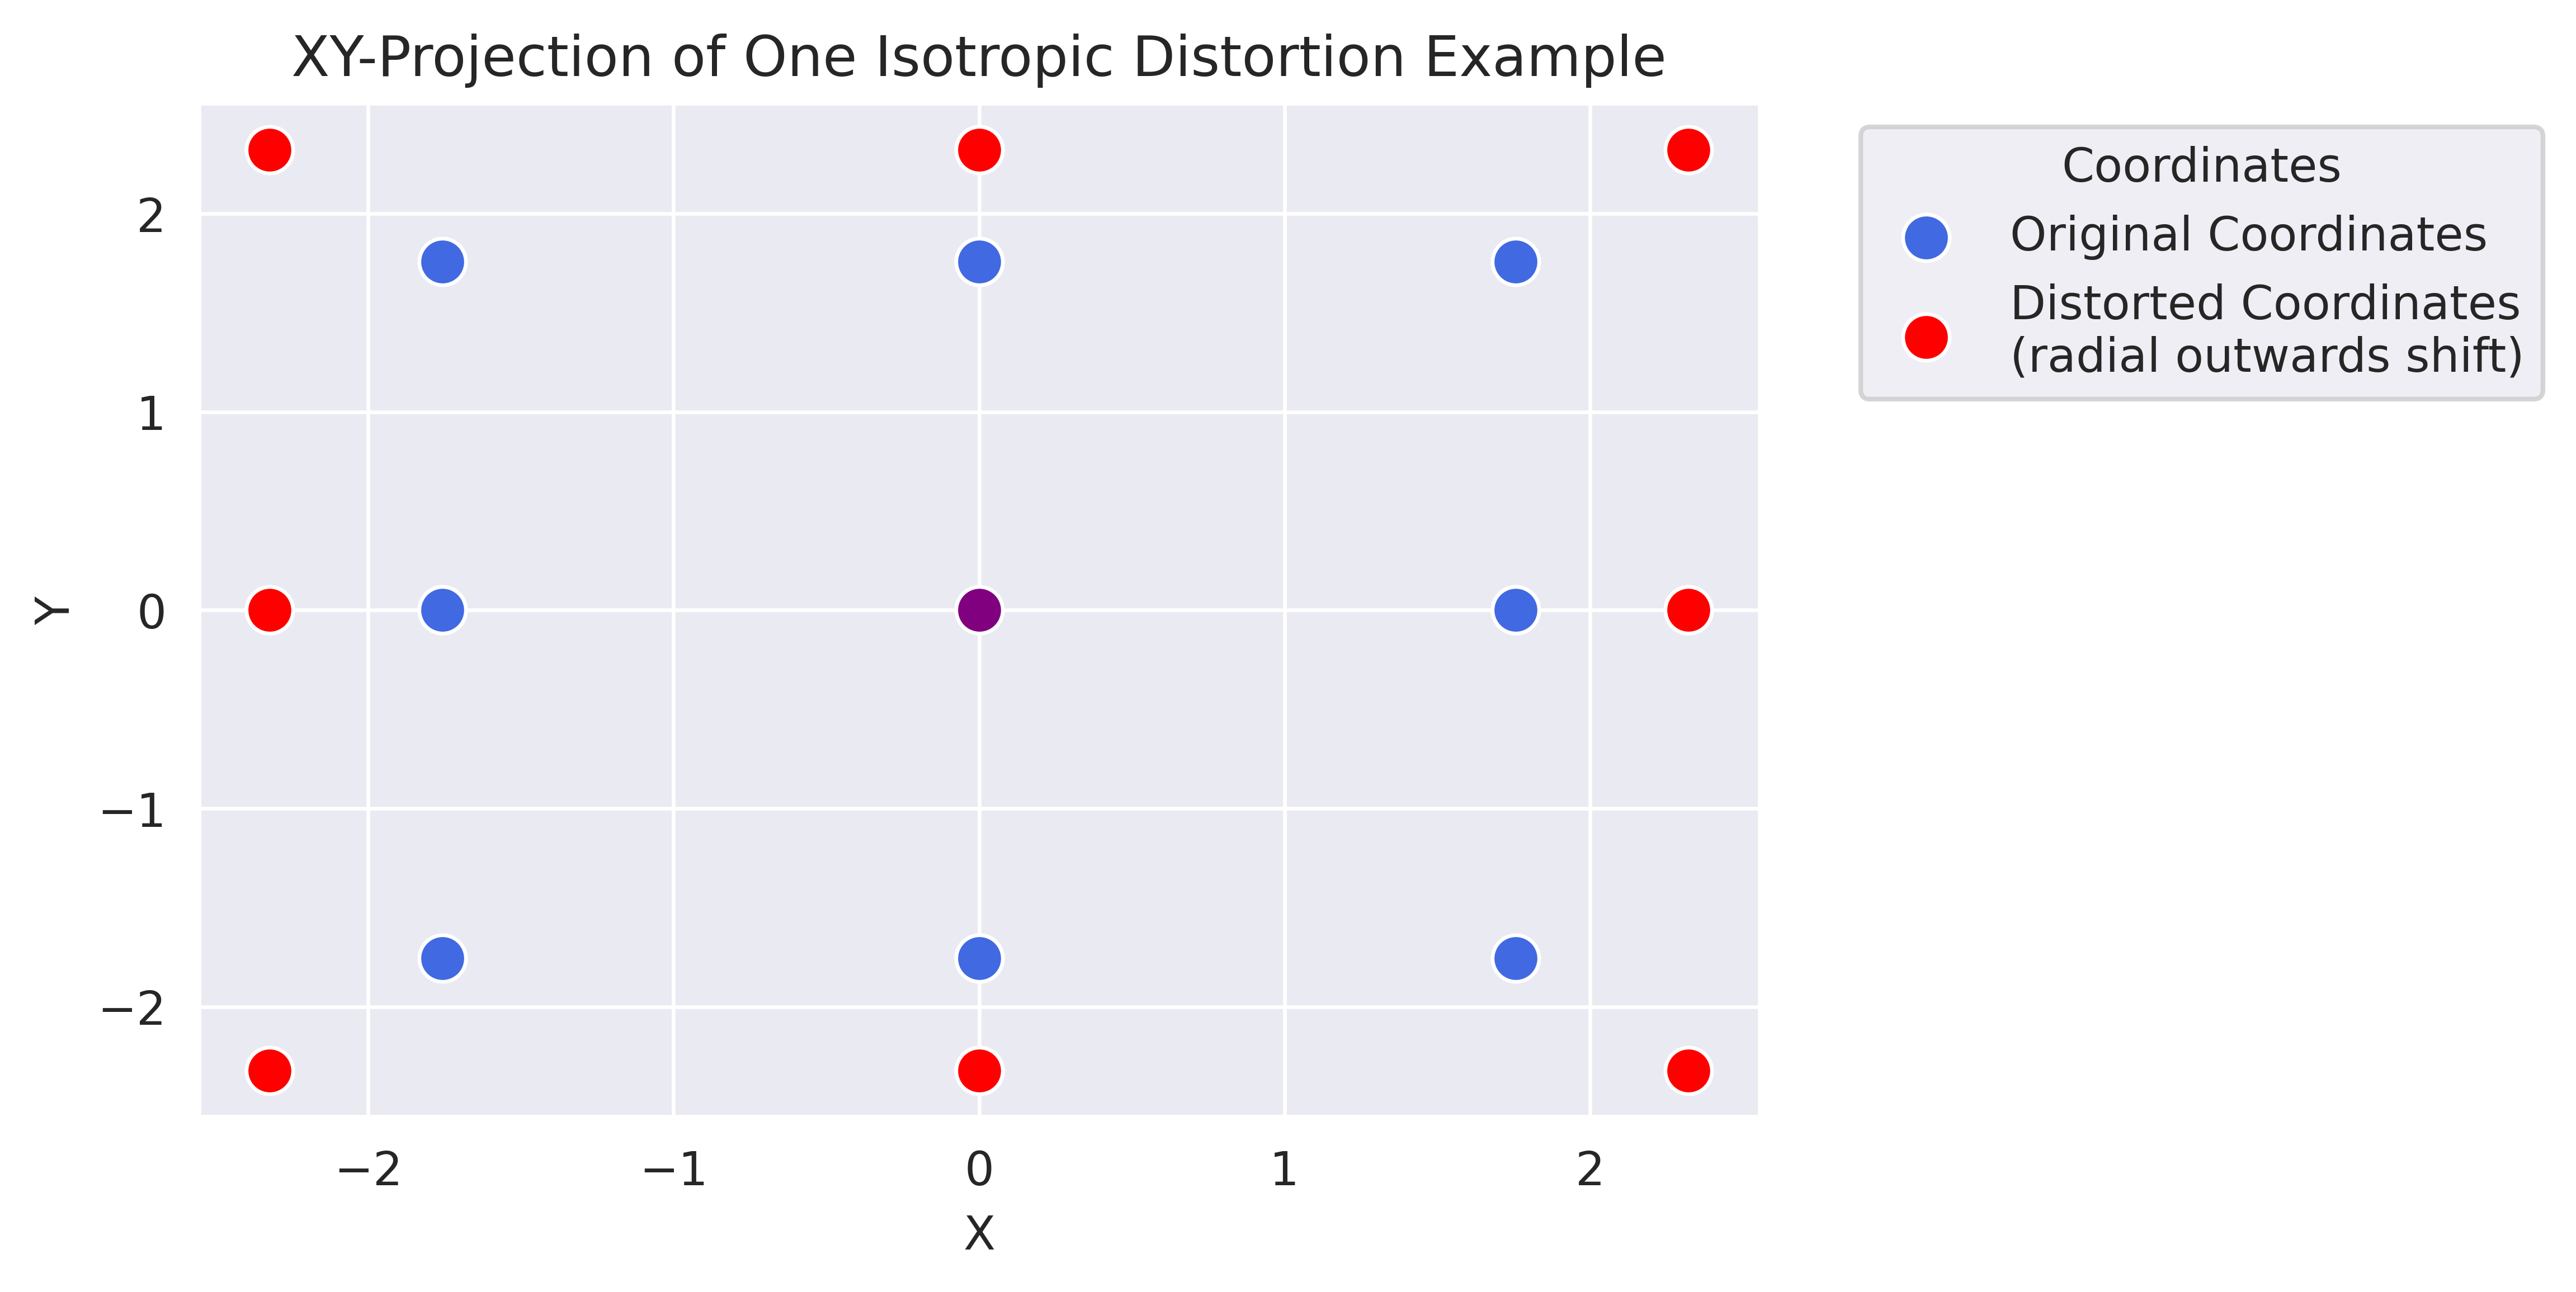
\includegraphics[width=\linewidth]{Chapters/Figures/2d_distortion_example.png}
	\caption[2D Distortion]{Each point represents an atom of an FCC unit cell projected onto the $xy$\nobreakdash-plane. The blue atoms represent the original coordinates, and the red atoms represent the radially shifted coordinates. The center absorber atom is purple since its original position is the same as its distorted position\todo[inline,color=yellow!40]{Is it fair to say this? Au is FCC, but FCC unit cells do not have a center. I am choosing a different point such that it actually looks more like BCC}}
	\label{fig:2d-distortion}
\end{figure}

Figure \ref{fig:2d-distortion} only shows the $xy$\nobreakdash-plane projection of the first 12 nearest neighbors, but the actual original structure consists of the first four shells (55 atoms) with a lattice constant of 
4.0782~\AA to match that of bulk Au. In reality, the nearest-neighbor distances for Au nanoparticles are likely smaller, \todo[color=green!40]{Citation? Wolfram Element Data?} but the important part is that the crystal structure is correct, especially since the original coordinates will only be one structure out of many.

A total of 91 FEFF input files are generated, each with the same center absorber located at $ (0,0,0) $ but with the other atomic coordinates in a shifted location. They are generated with shifts on the range of $ -0.45 $~\AA~to~$ +0.45 $~\AA~in increments of $ 0.01 $~\AA. For example, the FEFF input file with the greatest inward shift has coordinates shifted $ 0.45 $~\AA~radially inwards towards the center absorber, and the FEFF input file with the largest outwards shift has coordinates shifted $ 0.45 $~\AA~radially outwards away from the center absorber.

\begin{minipage}{\linewidth}
Each FEFF input file is run with the following parameters: 
\begin{Verbatim}[samepage=true, numbers=left]
    SCF 4.6 0 30 .5 1
    EDGE    L3
    EXCHANGE    5   0.2 0.5
    S02 1.
    XANES   3.7 0.05    0.1
    FMS 7

    POTENTIALS
    0	79	Au	-1	-1	0.
    1	79	Au	-1	-1	0.
\end{Verbatim}
~
\end{minipage}

Running the 91 simulations (one for each of the distorted structures) takes half an hour \todo[inline, color=blue!40]{I mention it because I want to make a point of how much computationally faster doing this XANES averaging process is}. The resulting XANES spectra are plotted in figure 

\begin{figure}[h]
	\centering
    \makebox[\textwidth][c]{
	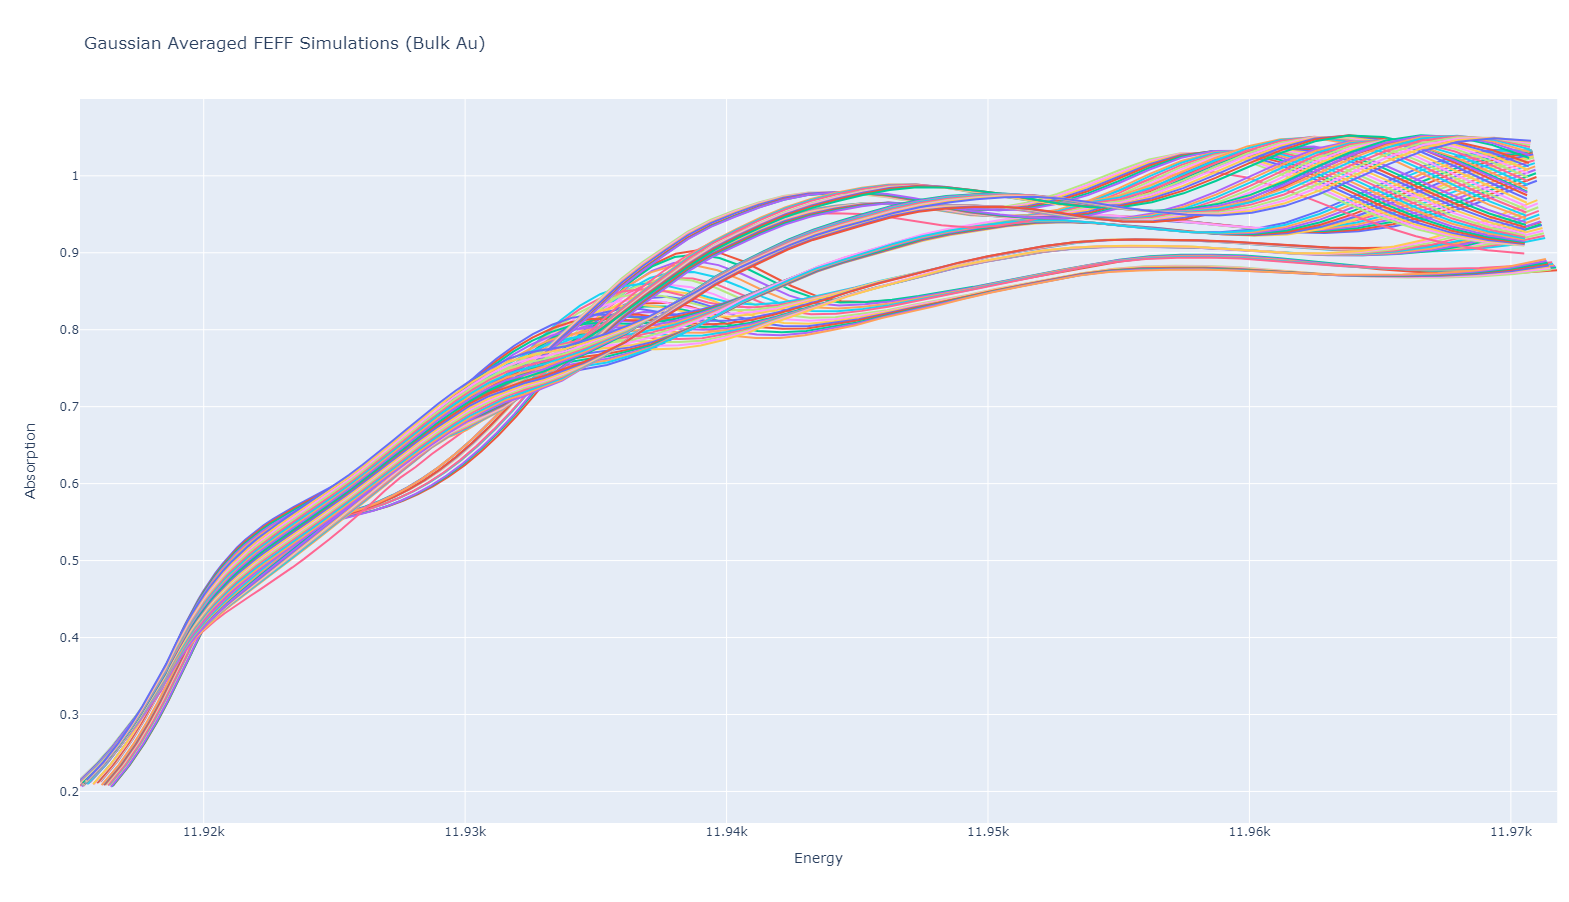
\includegraphics[width=1.1\linewidth]{Chapters/Figures/newplot.png}}
	\caption[FEFF Simulations Results]{TEMPORARY. Each spectrum represents the FEFF simulations result for a different distorted structure. That is to say, the crystal structure and center absorber are the same for each, the only parameter that varies is the euclidean distance from the center to the other coordinates.}
	\label{fig:feff-results}
\end{figure}

\section{Generating Disorder via Probability Distribution Averaging}

Disorder in a system can be characterized by the Gaussian width, sigma, of the partial radial distribution function. The idea of our statistical averaging method emulates/simulates this width by weighting the simulated XANES spectra accordingly. For example, figure \ref{fig:gaussian-weighting-hist} depicts a histogram with $ \sigma=0.1 $~\AA. Each histogram bin represents a simulated XANES spectrum with a different isotropic displacement. For example, the bin at $ \Delta\rho=0.0 $~\AA~represents the simulated XANES spectrum with no distortion, and the bin at $ \Delta\rho=-0.2 $~\AA~represents the simulated XANES spectrum with all the atomic coordinates shifted isotropically inwards towards the center absorber by $ 0.2 $~\AA. The height of each bin, $ f(\Delta\rho) $, represents the relative contribution of each simulated XANES spectrum towards the resulting weighted spectrum. For visual clarity, figure \ref{fig:gaussian-weighting-hist} depicts only 40 bins; the actual weighting includes 91 bins ranging from $ -0.45 $~\AA~to~$ +0.45 $~\AA~in increments of $ 0.01 $~\AA. \todo[color=pink!40]{Already mentioned earlier. Choose one.}

% figure created in playground.ipynb
% !htb
\begin{figure}[h!]
	\centering
	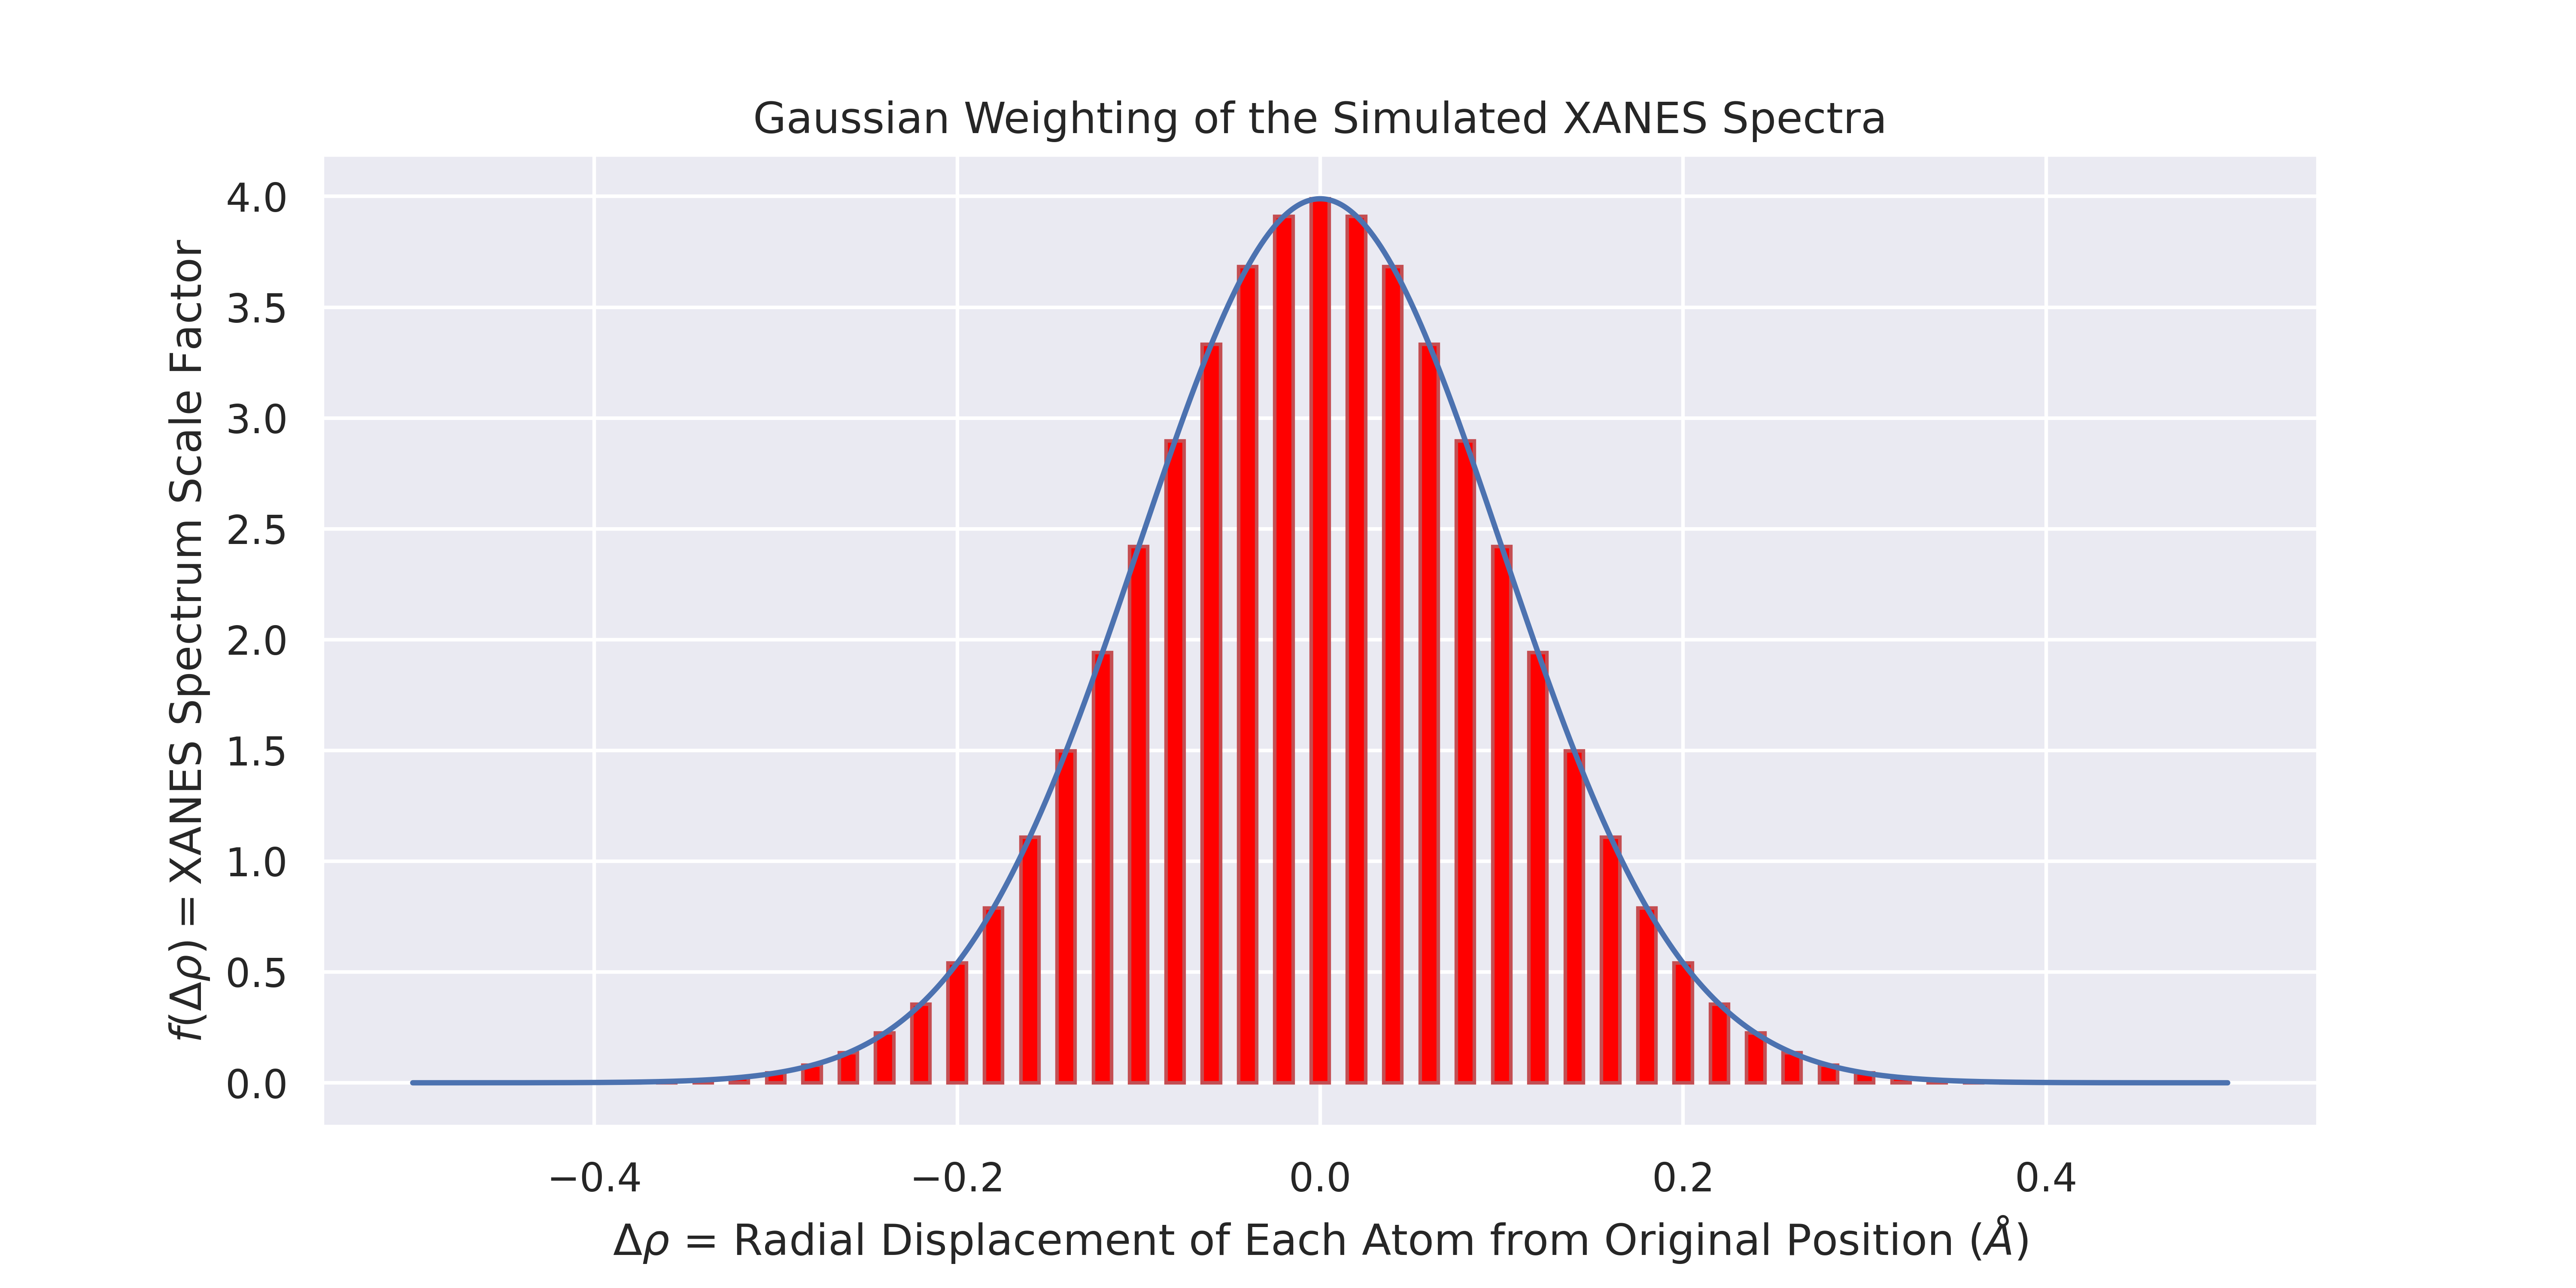
\includegraphics[width=\linewidth]{Chapters/Figures/gaussian-weighting-hist.png}
	\caption[Simulated Spectrum Gaussian Weighting]{A Gaussian distribution probability density function can be used to calculate the relative weight of each FEFF generated XANES spectrum towards one simulated, disordered spectrum. Each bin (red bar) represents a FEFF generated spectrum with the x-axis being the istropic shift of the atomic positions and the y-axis being the relative weight factor.}
	\label{fig:gaussian-weighting-hist}
\end{figure}

To calculate averaged XANES spectrum, $ \left\langle \mu(E) \right\rangle $, using the histogram weighting of the gaussian in figure \ref{fig:gaussian-weighting-hist}:

\begin{equation}
	\label{eqn:gaussian-averaging}
	\left\langle \mu(E) \right\rangle  = \frac{1}{S} \sum_{\Delta\rho=-.45}^{+.45} g\left(\Delta \rho \mid \mu=0, \sigma^2=0.01\right) \mu(E \mid \Delta\rho)
\end{equation}

\noindent
In the above equation $ \Delta\rho $ is the isotropic, radial displacement of each atom from their original positions and $ \mu(E \mid \Delta\rho) $ is the simulated FEFF spectrum for the given $ \Delta\rho $ configuration. Furthermore, (\ref{eqn:gaussian-averaging}), $ S $ represents a standardization factor to negate the effect of the changing height of the Gaussian as a function of the variance, $ \sigma^2 $. In this way, only the relative heights of each bin matter for producing the averaged XANES spectrum. The standardization factor, $ S $, can then be defined as:

\begin{equation}
	\label{eqn:gaussian-standardization}
	S = \sum_{\Delta\rho=-.45}^{+.45} g\left(\Delta \rho \mid \mu=0, \sigma^2=0.01\right)
\end{equation}

\noindent
In both equations \ref{eqn:gaussian-averaging} and \ref{eqn:gaussian-standardization}, the function $ g $ is just the typical Gaussian distribution probability density function: 

\begin{equation}
	\label{eqn:gaussian}
	g(x) = \frac{1}{{\sigma \sqrt {2\pi } }}e^{{{ - \left( {x - \mu } \right)^2 } \mathord{\left/ {\vphantom {{ - \left( {x - \mu } \right)^2 } {2\sigma ^2 }}} \right. \kern-\nulldelimiterspace} {2\sigma ^2 }}}
\end{equation}

The above example only generates one (simulated) disordered XANES spectrum and does so via weighting of a Gaussian distribution with mean and variance equal to $ 0 $ and $ 0.01 $, respectively. To simulate systems with different disorder, we can vary the shape of the probability density function. With a Gaussian distribution, we can only vary the mean and variance, but to simulate even more conditions, we can instead use the multivariate skew-normal distribution (eq \ref{eqn:skew-norm}) \cite{skewnorm_Azzalini_1999, 2020SciPy-NMeth}

\begin{equation}
	\label{eqn:skew-norm}
	f(x)=2\phi (x)\Phi (\alpha x)
\end{equation}
 
\noindent
where $ \phi(x) $ is the Gaussian PDF:
\begin{equation}
	\label{eqn:skew-norm-pdf}
	\phi (x)={\frac  {1}{{\sqrt  {2\pi }}}}e^{{-{\frac  {x^{2}}{2}}}}
\end{equation}

\noindent
and $ \Phi (x) $ is the Gaussian CDF:
\begin{equation}
	\label{eqn:skew-norm-cdf}
	\Phi (x)=\int _{{-\infty }}^{{x}}\phi (t)\ dt
\end{equation}

%------------WIKIPEDIA EQUATION VERSION -------------
% \begin{equation}
% 	\label{eqn:skew-norm-cdf}
% 	\Phi (x)=\int _{{-\infty }}^{{x}}\phi (t)\ dt={\frac  {1}{2}}\left[1+\operatorname {erf}\left({\frac  {x}{{\sqrt  {2}}}}\right)\right]
% \end{equation}
% \noindent
% and erf is Gauss' error-function

% \begin{equation}
% 	\label{eqn:skew-norm-cdf-erf}
% 	{\displaystyle \operatorname {erf} \left(z\right)={\frac {2}{\sqrt {\pi }}}\int _{0}^{z}e^{-t^{2}}\,dt}
% \end{equation}

\noindent
Equation \ref{eqn:skew-norm} includes the shape parameter, $ \alpha $, which has the nice properties of producing a right-skewed distribution when positive and a left-skewed distibution when negative. When $ \alpha=0 $ the distribution simply produces a the typical Gaussian distribution (eq. \ref{eqn:gaussian}). By using equation \ref{eqn:skew-norm}, we can vary $ \mu, \sigma,  $ and $ \alpha $ to vary the first four moments of the function: mean, standard deviation, skew, and kurtosis. Eighteen possible skew-norm weighting functions are plotted in Figure \ref{fig:skew-norm-options}. 

\begin{figure}[h!]
	\centering
	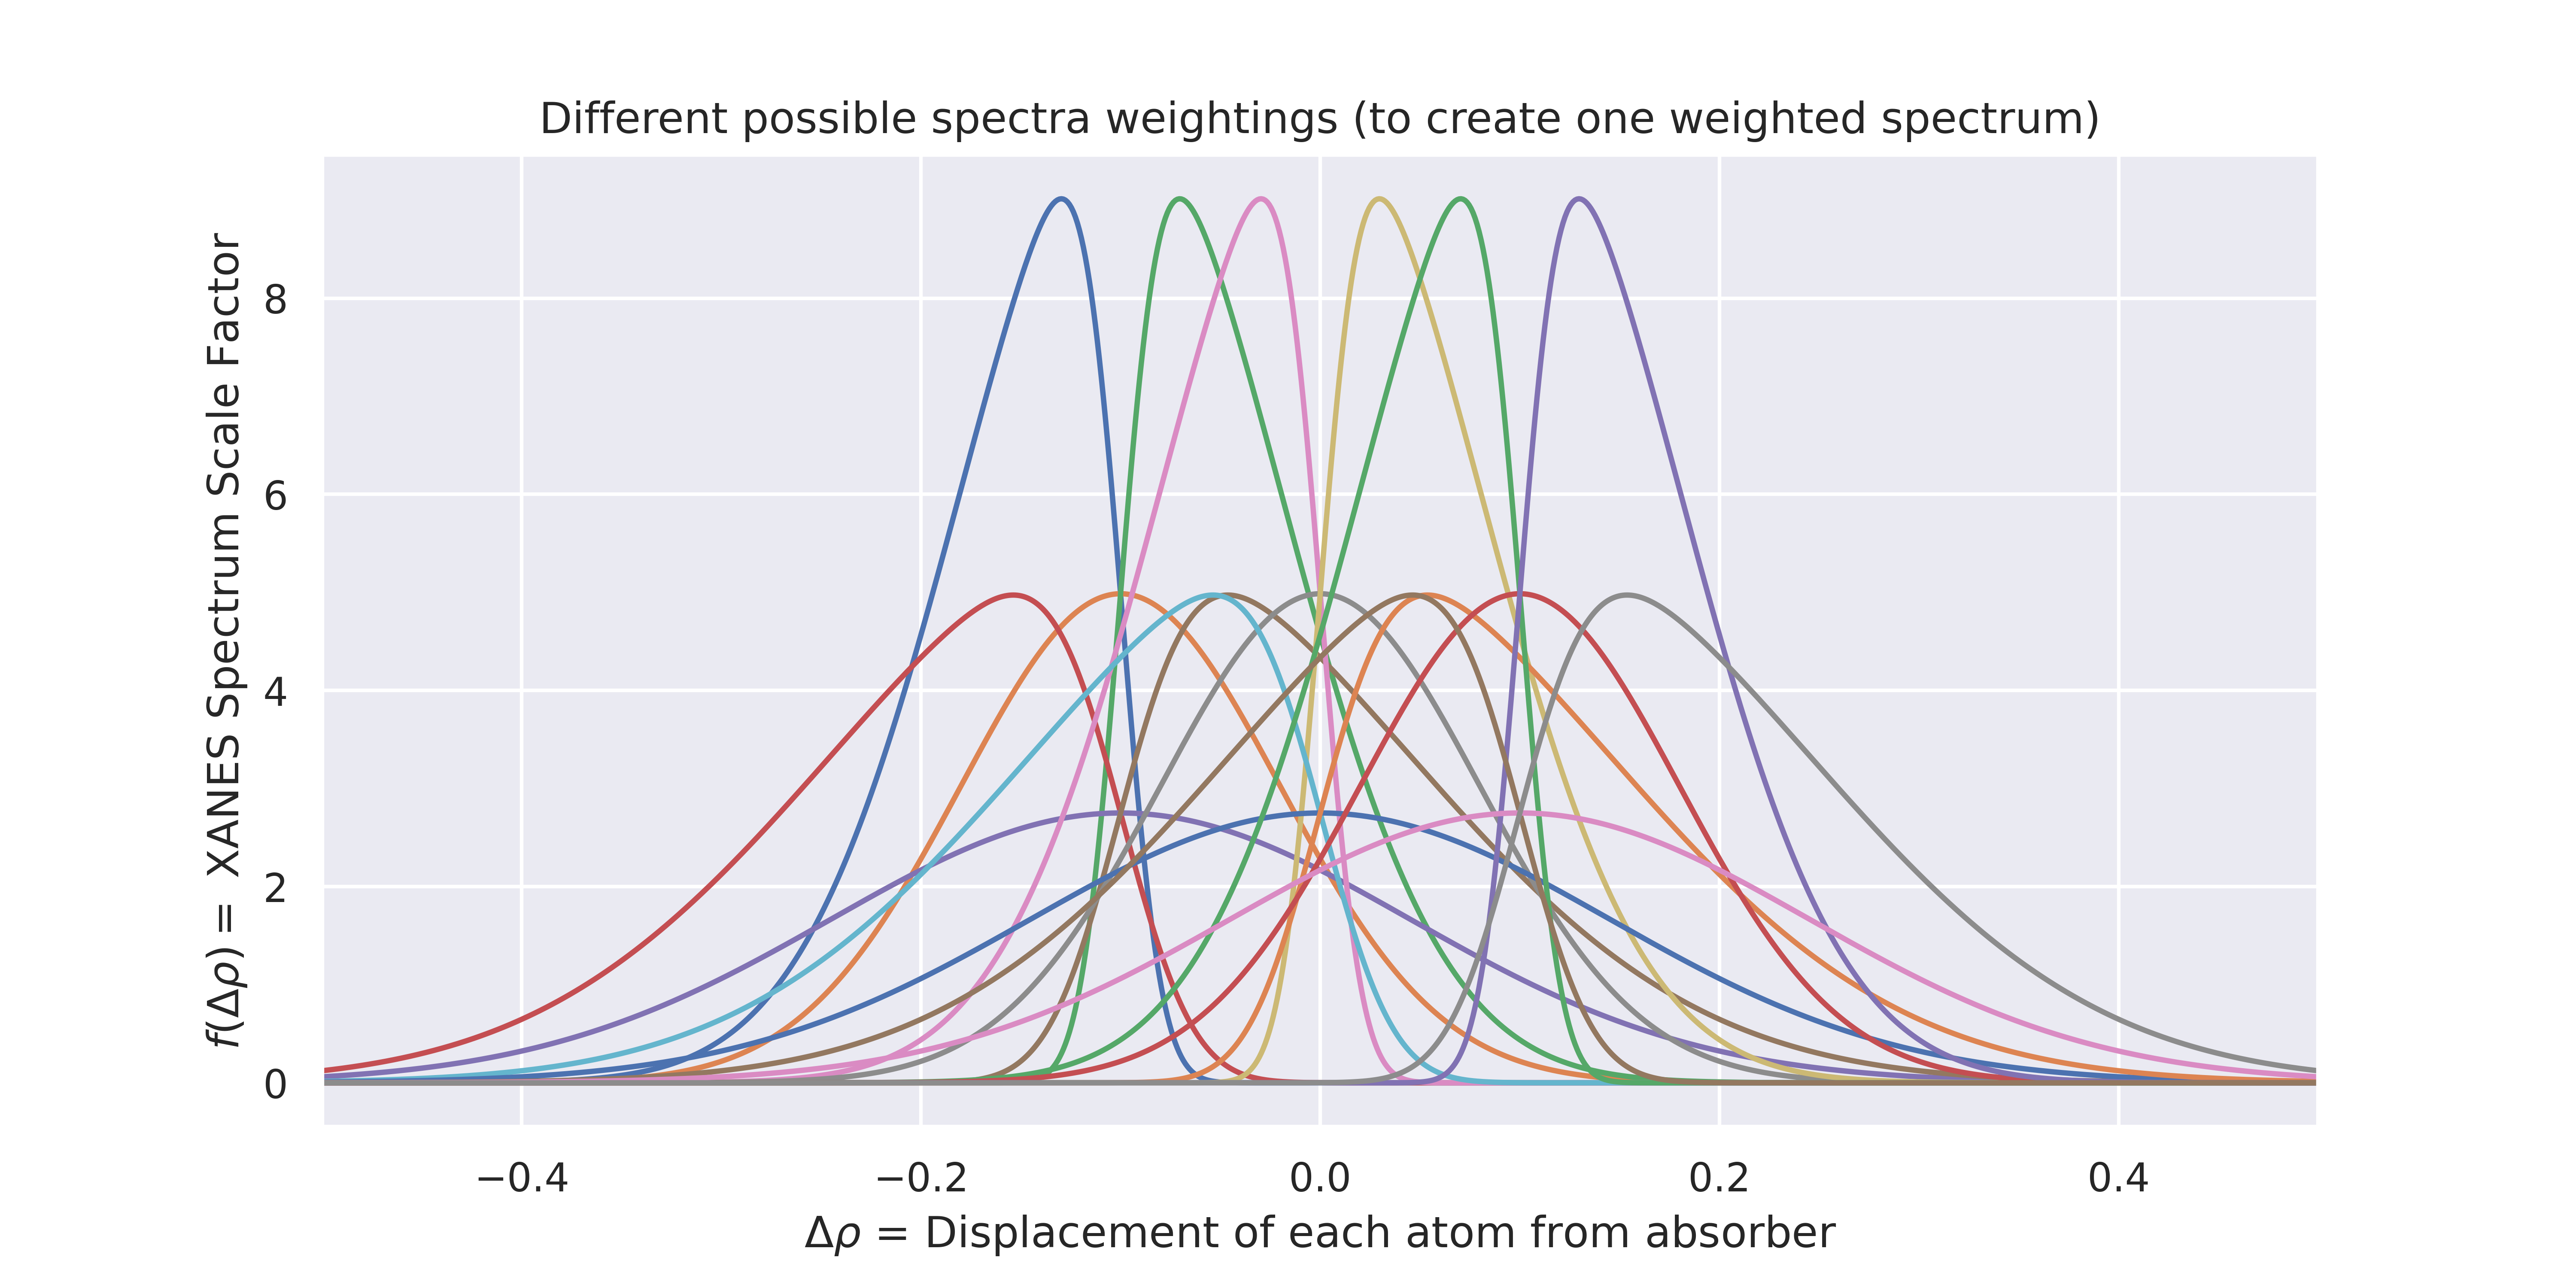
\includegraphics[width=\linewidth]{Chapters/Figures/skewnorm_options.png}
	\caption[Simulated Disordered Spectrum Weightings]{Eighteen skew-norm functions are plotting with all possible permutations of $ \sigma=\{.08, .145\} $, $ \mu=\{-.1, 0, .1\} $, and $ \alpha=\{-5,0,5\} $.}
	\label{fig:skew-norm-options}
\end{figure}


\section{Simulation vs. Experimental Data}

\begin{figure}[h]
	\centering
	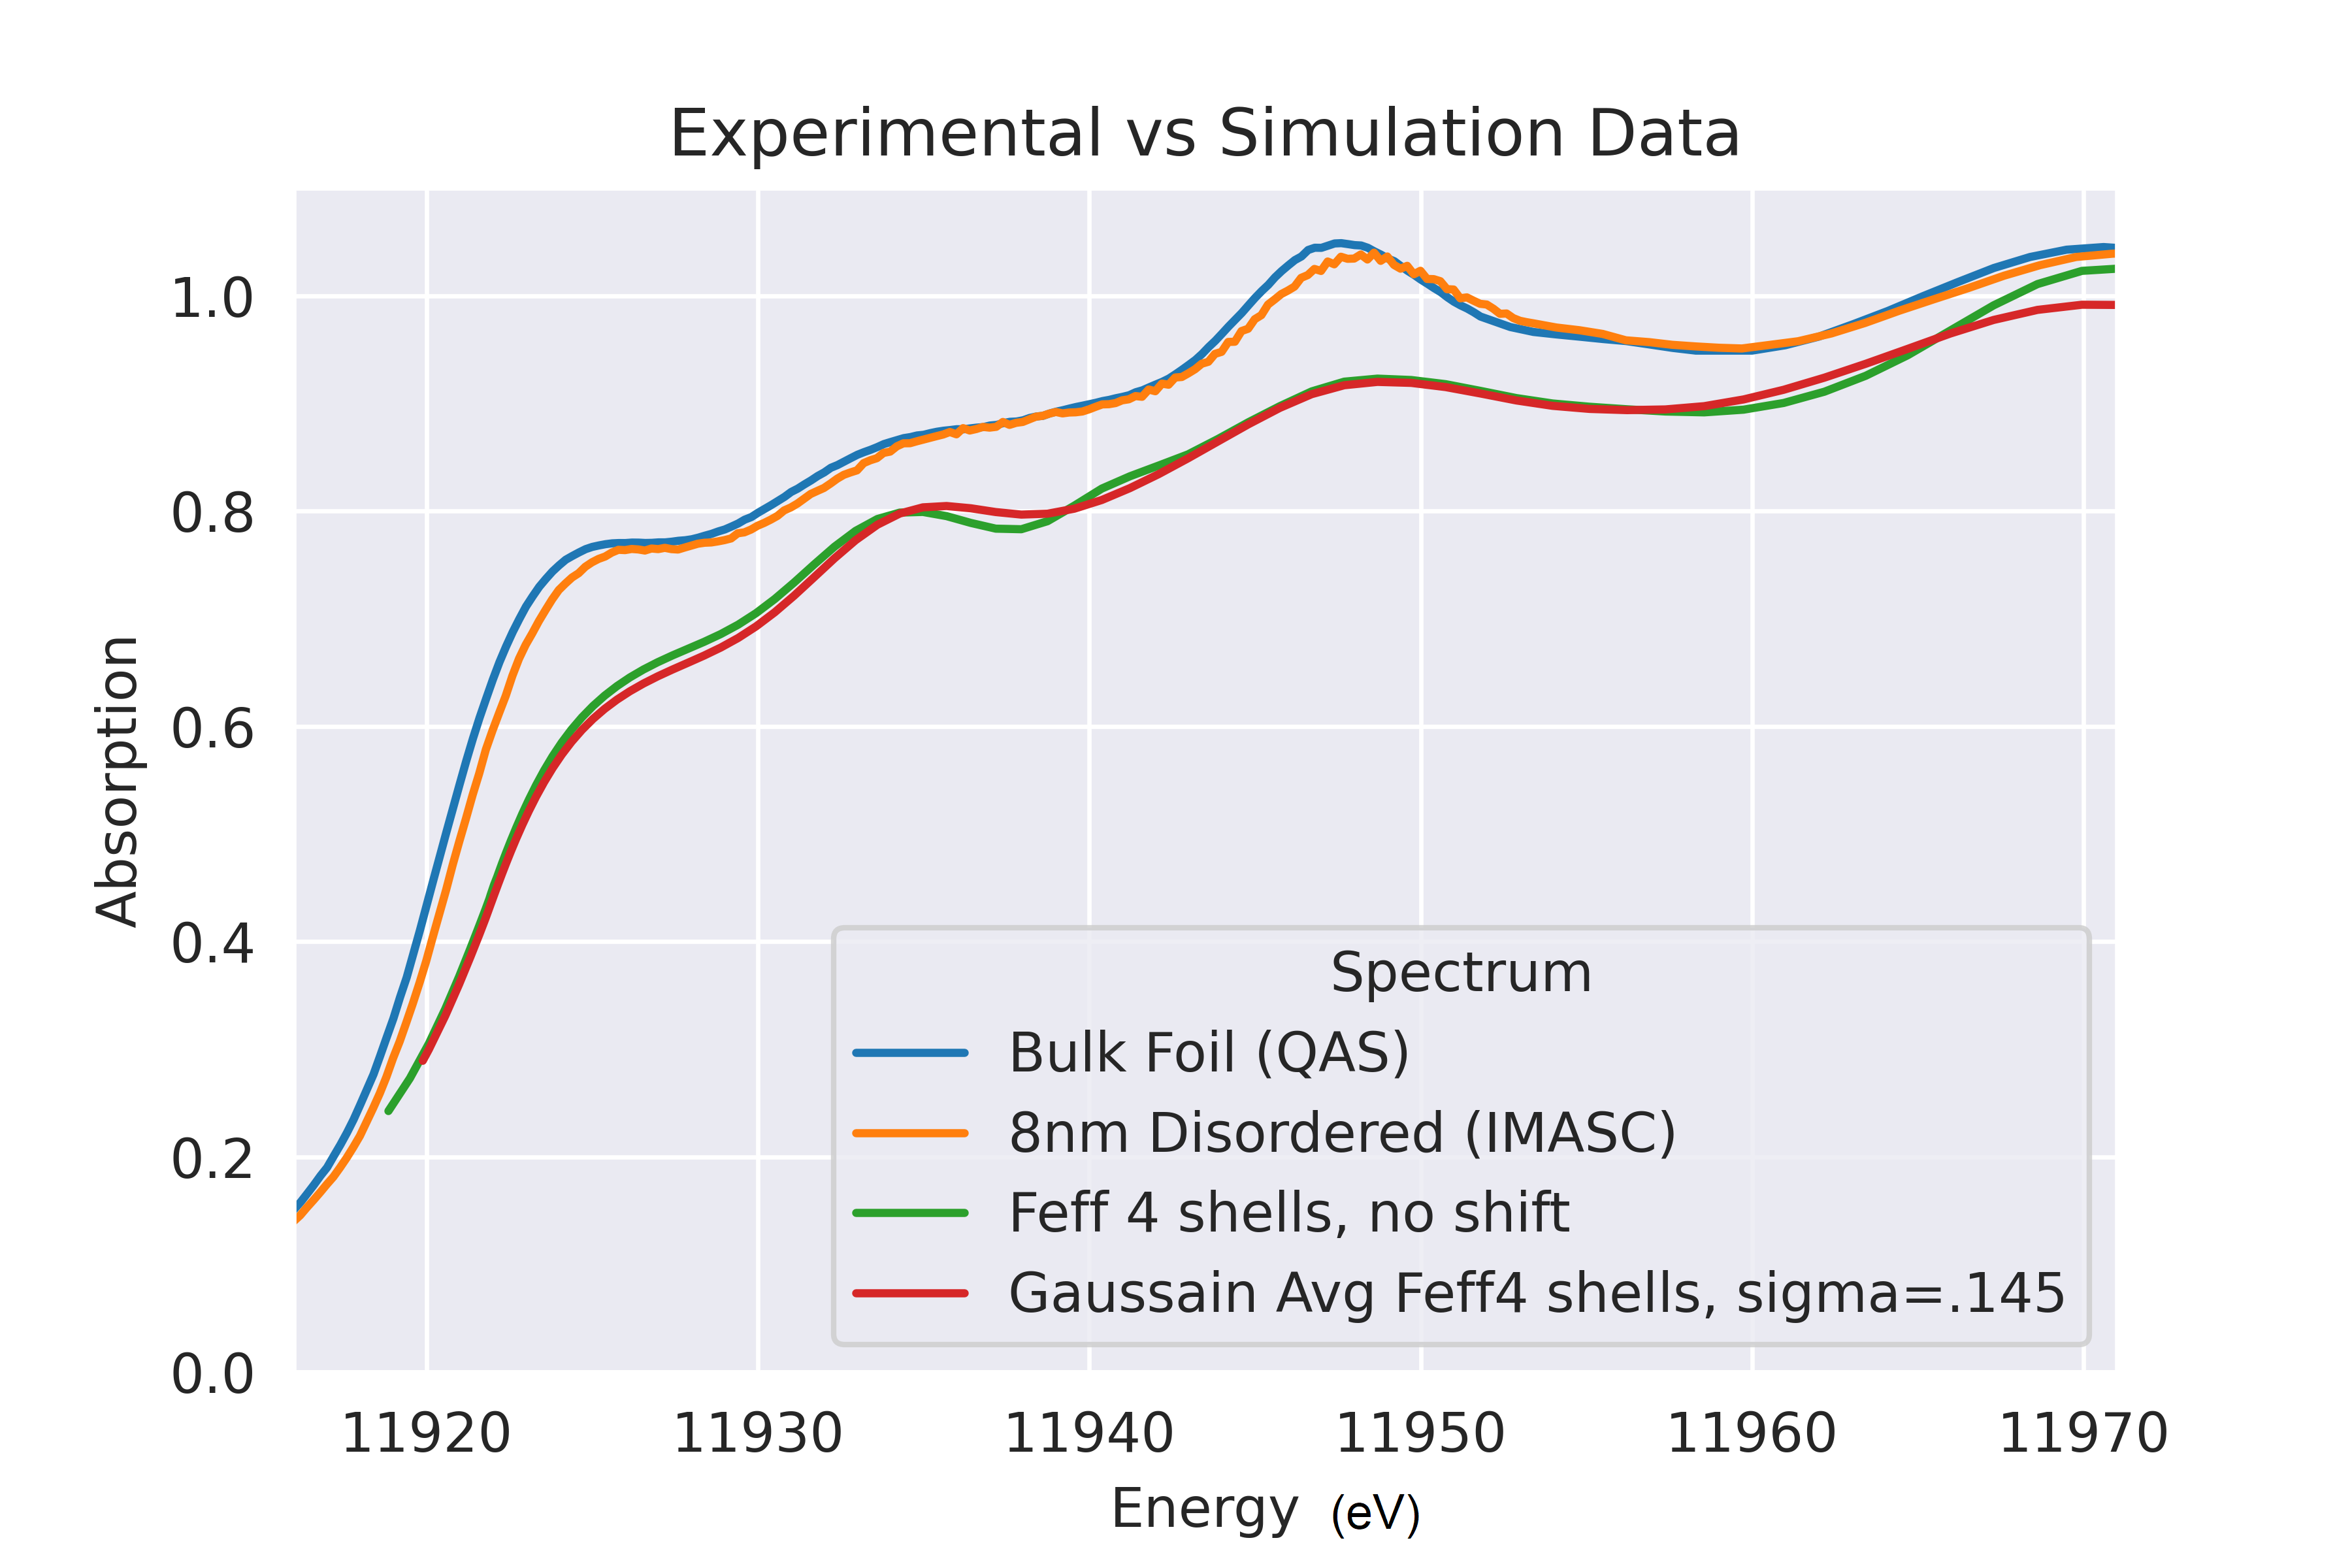
\includegraphics[width=.7\linewidth]{Chapters/Figures/bulk_8nm_disorder_experimental_theory_comparison.png}
	\caption[Simulation vs. Experimental]{TEMPORARY CAPTION}
	\label{fig:avg-experimental-vs-simulation}
\end{figure}


\begin{figure}[h]
	\centering
	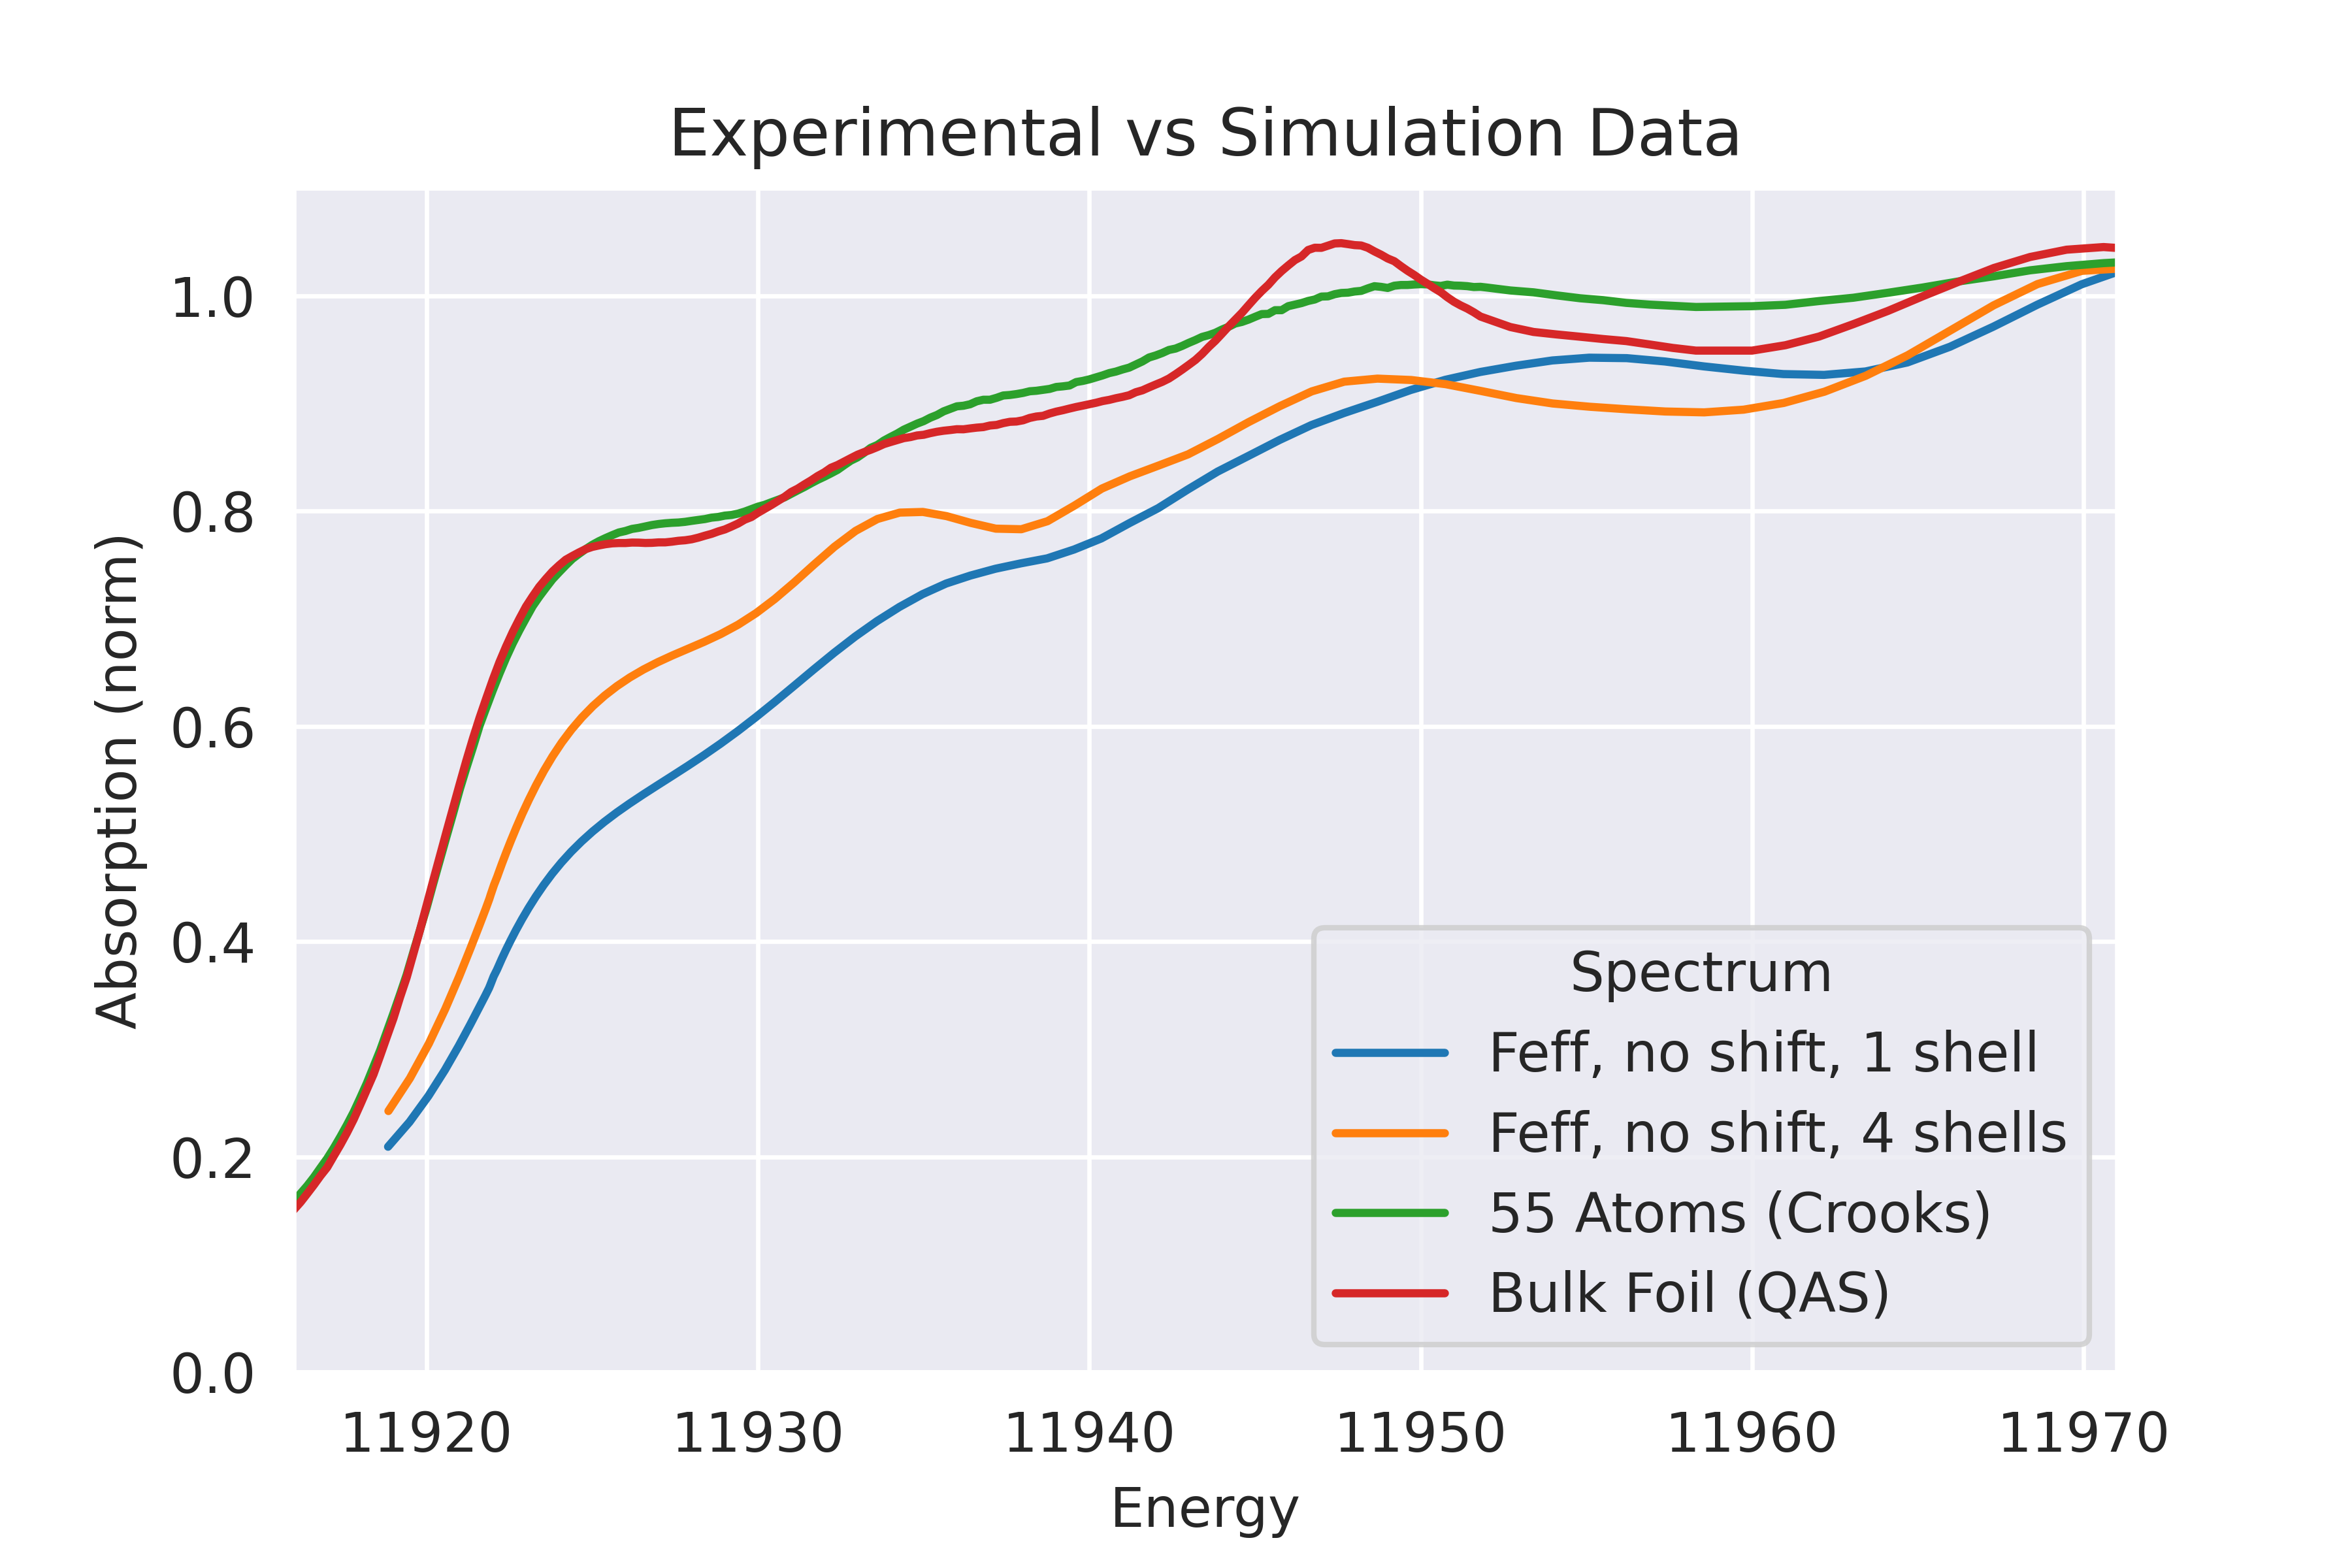
\includegraphics[width=.7\linewidth]{Chapters/Figures/Bulk_55atom_experimental_theory_comparison.png}
	\caption[Simulation vs. Experimental 2]{TEMPORARY CAPTION}
	\label{fig:avg-experimental-vs-simulation2}
\end{figure}


